% 2010 new-curriculum science q4 option D (distractor, schematic): d = 2|cos 2t|, t in [0,2pi];
% starts at 2, first zero at pi/4, period pi/2, maxima 2.
% Source: inputs/original_02.pdf p.1 (option D bitmap, img/2010/new_curriculum_science/q4_optD.png).
\usetikzlibrary{arrows.meta}
\begin{tikzpicture}[x=0.9cm,y=0.9cm,line width=.6pt,font=\normalsize,>=Stealth]
\draw[->] (-1,0)--(7,0) node[anchor=west,inner sep=0pt,xshift=2pt] {$x$};
\draw[->] (0,-1)--(0,3) node[anchor=south,inner sep=0pt,yshift=2pt] {$y$};
\draw[domain=0:6.2832,samples=360] plot (\x,{2*abs(cos(deg(2*\x)))});
\draw (-0.1,2)--(0.15,2);
\node[anchor=east,inner sep=1pt,xshift=-2pt] at (-0.12,2) {$2$};
\node[anchor=north,inner sep=1pt,yshift=-1pt] at (0.7854,0) {$\dfrac{\pi}{4}$};
\node[below left,inner sep=1pt] at (0,0) {$O$};
\end{tikzpicture}
